\chapter{Quỹ đạo photon, không gian Rindler và phần trong Schwarzschild}

Một khối lượng điểm Newton và một lỗ đen Schwarzschild bắt đầu từ cùng một sự lý tưởng hóa: toàn bộ khối lượng gây hấp dẫn đều tập trung ở tâm. Tuy vậy, tâm của chúng lại mang những ý nghĩa rất khác nhau. Trong cơ học Newton, một hạt dù chỉ có một chút mômen động lượng cũng sẽ không đi trúng tâm. Trong lỗ đen, một khi hạt đã vượt qua chân trời, không thể không chạm tới kỳ dị. Để hiểu sự khác biệt đó, ta sẽ đi qua các quỹ đạo tròn, mặt cầu photon, và cuối cùng là một hệ tọa độ mới gần chân trời.

\section{Một tâm không thể nào tránh được}

Vật chất thực trong cơ học Newton không bao giờ trở thành một điểm toán học. Áp suất, độ bền vật liệu và các lực khác chống lại sự nén. Ngay cả nếu ta vẫn dùng khối lượng điểm như một sự lý tưởng hóa, một hạt rơi vào cũng hiếm khi va trúng nó. Một quỹ đạo chính xác theo phương bán kính có thể tới \(r=0\), nhưng chỉ một vận tốc ngang nhỏ nhất cũng cung cấp mômen động lượng. Khi đó rào cản ly tâm bẻ quỹ đạo của hạt đi vòng quanh tâm.

Thuyết tương đối rộng làm thay đổi kết luận ấy. Một vật thể đủ đặc có thể hình thành lỗ đen, và miền trong của lỗ đen triệt tiêu lối thoát kiểu Newton bằng con đường đi vòng quanh tâm. Lý do còn sâu hơn chuyện lực mạnh hơn: bên trong chân trời, giảm \(r\) là một hướng về tương lai. Ta sẽ đi tới phát biểu đó từng bước thay vì giả định trước.

\begin{classroomqa}
\audiencequestion{Phải chăng khó khăn theo Newton trong việc chạm tới tâm chỉ đơn thuần là hệ quả của việc coi cả hai vật như những điểm?}
\lecturerresponse{Sự lý tưởng hóa thành điểm là một phần của phép so sánh, nhưng đó không phải toàn bộ sự khác biệt. Trong cơ học Newton, bất kỳ mômen động lượng khác không nào cũng cho phép quỹ đạo lượn quanh điểm đó. Trong miền trong tương đối tính, kỳ dị nằm về phía tương lai của mọi quỹ đạo kiểu thời gian đang rơi vào; chuyển động góc không thể đem lại một lối thoát.
\lecturetimestamp{00:04:52--00:05:13}}
\end{classroomqa}

\section{Chân trời và kỳ dị}

Tạm thời ta coi hình học Schwarzschild là đã cho:
\begin{equation}
d\tau^{2}
=
\left(1-\frac{2MG}{r}\right)dt^{2}
-
\frac{dr^{2}}{1-\frac{2MG}{r}}
-
r^{2}d\Omega^{2}.
\label{eq:l6-schwarzschild}
\end{equation}
Các phương trình trường chọn ra metric này sẽ được trình bày sau. Nhiệm vụ trước mắt của ta là hiểu metric ấy nói gì.

Ta có thể viết metric trên mặt cầu đơn vị là
\begin{equation}
d\Omega^{2}
=d\vartheta^{2}+\cos^{2}\vartheta\,d\phi^{2}
\label{eq:l6-angular-metric}
\end{equation}
khi \(\vartheta\) là vĩ độ đo từ mặt phẳng xích đạo. Với góc cực quen thuộc hơn, đo từ trục, cosine trở thành sine. Đối xứng cầu cho phép đặt mọi quỹ đạo vào một mặt phẳng cố định, nên trong phép tính dưới đây chỉ còn lại một tọa độ góc.

\begin{figure}[htbp]
\centering
\includegraphics[width=0.88\textwidth]{lecture_06_figure_01.png}
\caption{Metric Schwarzschild và hình dung không-thời gian hình trụ của mặt \(r=2MG\). Đường thẳng ở tâm là \(r=0\); trụ đỏ là chân trời trong tọa độ Schwarzschild.}
\lectureframe{00:09:45}
\end{figure}

Ở xa nguồn, \(2MG/r\) nhỏ và Phương trình~\eqref{eq:l6-schwarzschild} tiến tới metric Minkowski trong tọa độ cầu. Có hai bán kính nổi bật:
\begin{equation}
r=2MG,
\qquad
r=0.
\end{equation}
Không được nhầm lẫn chúng. Tại \(r=2MG\), hệ số của \(dt^{2}\) triệt tiêu còn hệ số của \(dr^{2}\) phân kỳ. Hệ tọa độ Schwarzschild đã trở nên kỳ dị. Bản thân độ cong vẫn hữu hạn ở đó. Trái lại, tại \(r=0\), các bất biến độ cong phân kỳ. Trường thủy triều kéo giãn một vật có kích thước theo phương bán kính và ép nó theo phương ngang một cách vô hạn. Đó là một kỳ dị vật lý, không phải một khuyết tật của tọa độ.

\subsection{Hai cách đo thời gian của sự rơi}

Đối với một đồng hồ đứng yên bên ngoài chân trời,
\begin{equation}
d\tau
=
\sqrt{1-\frac{2MG}{r}}\,dt.
\label{eq:l6-static-clock}
\end{equation}
Khi \(r\) lớn, \(d\tau\simeq dt\). Gần chân trời, thời gian riêng của một đồng hồ được giữ ở \(r\) cố định trôi rất chậm so với thời gian Schwarzschild đo ở xa.

Cùng các tọa độ ấy, sự rơi theo phương bán kính được mô tả là cần một giá trị vô hạn của \(t\) để tới \(r=2MG\). Thời gian riêng trôi qua của chính vật rơi thì hữu hạn. Giữa hai phát biểu đó không có mâu thuẫn. Một đồng hồ do vật rơi mang theo đo thời gian riêng dọc theo đường thế giới của nó. Đó có thể là đồng hồ cơ, một đồng hồ ánh sáng tạo bởi các gương ở hai đầu một thanh thước mét, một nhịp tim, hoặc chuỗi các quá trình vật lý trong não. Không cái nào trong số đó đo tọa độ \(t\) ở xa. Sự phân biệt giữa hai đồng hồ sẽ hiện ra trong giản đồ gần chân trời.

\section{Chuyển động tròn từ tác dụng theo thời gian riêng}

Trước khi trở lại bài toán rơi vào, ta hãy giải một vấn đề khác: trong những điều kiện nào thì một hạt có khối lượng hoặc một photon có thể chuyển động tròn quanh lỗ đen? Phép tính bắt đầu từ cùng nguyên lý tác dụng dùng cho mọi hạt tương đối tính chuyển động tự do,
\begin{equation}
S=-m\int d\tau.
\label{eq:l6-particle-action}
\end{equation}
Ánh sáng bị Trái Đất bẻ cong, nhưng trường hấp dẫn của nó hoàn toàn không đủ mạnh để uốn một tia sáng thành một quỹ đạo. Bán kính Schwarzschild của Trái Đất chỉ cỡ một xentimét. Ta sẽ phải nén toàn bộ Trái Đất xuống xấp xỉ thang đó, cỡ một quả hạch nhỏ, thì câu hỏi về trường mạnh mới trở nên thích hợp.

Đặt \(c=1\), giới hạn chuyển động trong một mặt phẳng xích đạo, và định nghĩa
\begin{equation}
F(r)=1-\frac{2MG}{r},
\qquad
G(r)=\frac{1}{F(r)}.
\label{eq:l6-fg}
\end{equation}
Dùng thời gian tọa độ \(t\) làm tham số, ta được
\begin{equation}
d\tau
=dt\sqrt{F-G\dot r^{\,2}-r^{2}\dot\theta^{\,2}},
\end{equation}
và do đó
\begin{equation}
\mathcal L
=
-m\sqrt{F-G\dot r^{\,2}-r^{2}\dot\theta^{\,2}}.
\label{eq:l6-lagrangian}
\end{equation}
Thừa số \(m\) làm cho tác dụng có thứ nguyên thông thường là năng lượng nhân thời gian.

\begin{figure}[htbp]
\centering
\includegraphics[width=0.76\textwidth]{lecture_06_figure_02.png}
\caption{Lagrangian căn bậc hai của hạt đang được ghép lại trên bảng. Biểu thức đầy đủ được cho trong Phương trình~\eqref{eq:l6-lagrangian}.}
\lectureframe{00:31:53}
\end{figure}

Với mọi tọa độ suy rộng \(q\),
\begin{equation}
p_q=\frac{\partial\mathcal L}{\partial\dot q}.
\end{equation}
Sẽ hữu ích nếu dành \(\mathcal L\) cho Lagrangian và \(L\) cho mômen động lượng. Với
\begin{equation}
\Delta=F-G\dot r^{\,2}-r^{2}\dot\theta^{\,2},
\end{equation}
hai xung lượng là
\begin{align}
L=p_\theta
&=\frac{mr^{2}\dot\theta}{\sqrt{\Delta}},
\label{eq:l6-angular-momentum}\\
p_r
&=\frac{mG\dot r}{\sqrt{\Delta}}.
\label{eq:l6-radial-momentum}
\end{align}
Xung lượng theo phương bán kính không được bảo toàn vì tọa độ bán kính xuất hiện trong Lagrangian. Góc \(\theta\) không xuất hiện, nên \(L\) được bảo toàn.

Cũng không có \(t\) tường minh trong \(\mathcal L\). Vì thế Hamiltonian được bảo toàn:
\begin{align}
E=H
&=p_r\dot r+L\dot\theta-\mathcal L \\
&=\frac{mG\dot r^{\,2}}{\sqrt{\Delta}}
  +\frac{mr^{2}\dot\theta^{\,2}}{\sqrt{\Delta}}
  +m\sqrt{\Delta} \\
&=\frac{mF}{\sqrt{\Delta}}.
\label{eq:l6-energy-general}
\end{align}
Đây là một nhịp điệu đặc trưng của cơ học. Một nguyên lý cho tác dụng; một phép tính cho các xung lượng; rồi đối xứng lại biến phép tính ấy trở về các định luật bảo toàn năng lượng và mômen động lượng. Ta có thể lập tức giải tất cả các phương trình Euler--Lagrange, nhưng các hằng số do đối xứng quay và đối xứng tịnh tiến theo thời gian cung cấp loại bỏ được phần lớn công việc đó.

\subsection{Năng lượng của quỹ đạo tròn}

Đối với một quỹ đạo tròn,
\begin{equation}
\dot r=0.
\end{equation}
Đưa vào mômen động lượng trên đơn vị khối lượng,
\begin{equation}
\lambda=\frac{L}{m}.
\end{equation}
Các phương trình~\eqref{eq:l6-angular-momentum} và
\eqref{eq:l6-energy-general} trở thành
\begin{align}
\lambda
&=\frac{r^{2}\dot\theta}
{\sqrt{F-r^{2}\dot\theta^{\,2}}},
\label{eq:l6-lambda-circular}\\
E
&=\frac{mF}{\sqrt{F-r^{2}\dot\theta^{\,2}}}.
\label{eq:l6-energy-circular-first}
\end{align}

\begin{figure}[htbp]
\centering
\includegraphics[width=0.82\textwidth]{lecture_06_figure_04.png}
\caption{Mômen động lượng trên đơn vị khối lượng và năng lượng cho chuyển động tròn Schwarzschild. Trước hết dùng phương trình mômen động lượng để khử \(\dot\theta\) khỏi năng lượng.}
\lectureframe{00:39:14}
\end{figure}

Bình phương Phương trình~\eqref{eq:l6-lambda-circular} và giải theo vận tốc góc cho
\begin{equation}
\dot\theta^{\,2}
=
\frac{\lambda^{2}F}
{r^{2}\left(r^{2}+\lambda^{2}\right)}.
\label{eq:l6-angular-speed}
\end{equation}
Thế vào Phương trình~\eqref{eq:l6-energy-circular-first}, ta còn lại một năng lượng chỉ phụ thuộc vào bán kính giả định và mômen động lượng cố định:
\begin{equation}
E(r,\lambda)
=m\sqrt{F(r)}\,\frac{\sqrt{r^{2}+\lambda^{2}}}{r}.
\label{eq:l6-circular-energy}
\end{equation}

Cả lớp dừng lại để so sánh với Newton. Trong một quỹ đạo tròn thông thường, tần số góc và tốc độ tiếp tuyến giảm khi bán kính tăng, nhưng mômen động lượng còn chứa một thừa số bán kính. Vì vậy không nên suy ra sự biến thiên của \(L\) chỉ từ tốc độ góc. Công thức tương đối tính giữ các thừa số ấy tường minh.

\section{Quỹ đạo tròn của ánh sáng}

Một photon có năng lượng và động lượng mặc dù nó không có khối lượng nghỉ. Vì vậy, giới hạn không khối lượng của Phương trình~\eqref{eq:l6-circular-energy} phải được lấy một cách cẩn thận. Nếu \(m\) tiến về không khi giữ \(\lambda\) cố định, thì \(L=m\lambda\) cũng sẽ triệt tiêu. Thay vào đó, lấy
\begin{equation}
m\longrightarrow0,
\qquad
\lambda\longrightarrow\infty,
\qquad
L=m\lambda\ \text{fixed}.
\label{eq:l6-massless-limit}
\end{equation}
Khi ấy hạng \(\lambda^{2}\) chi phối, và năng lượng của photon trở thành
\begin{equation}
E_\gamma(r;L)
=L\,\frac{\sqrt{1-\frac{2MG}{r}}}{r}.
\label{eq:l6-photon-energy}
\end{equation}
Thừa số \(L\) nhân với toàn bộ hàm theo bán kính. Nó ảnh hưởng đến thang năng lượng nhưng không ảnh hưởng đến bán kính của quỹ đạo tròn.

\begin{figure}[htbp]
\centering
\includegraphics[width=0.88\textwidth]{lecture_06_figure_05.png}
\caption{Nhân tử theo bán kính trong năng lượng của photon. Nó triệt tiêu tại chân trời, giảm dần về không ở bán kính lớn, và có một cực đại giữa hai nơi ấy.}
\lectureframe{00:50:50}
\end{figure}

Với \(L\) cố định, cân bằng theo phương bán kính đòi hỏi một điểm dừng:
\begin{equation}
\frac{d}{dr}
\left[
\frac{\sqrt{1-\frac{2MG}{r}}}{r}
\right]=0.
\end{equation}
Lấy đạo hàm,
\begin{equation}
-\frac{\sqrt{1-\frac{2MG}{r}}}{r^{2}}
+
\frac{MG}
{r^{3}\sqrt{1-\frac{2MG}{r}}}
=0,
\end{equation}
và do đó
\begin{equation}
r=3MG.
\label{eq:l6-photon-sphere}
\end{equation}
Bán kính này lớn gấp rưỡi bán kính Schwarzschild. Nó thường được gọi là mặt cầu photon.

Điểm dừng ấy là một cực đại, nên quỹ đạo tròn của photon là không ổn định. Một photon được đặt đúng tại \(3MG\) sẽ ở lại đó. Một độ dời theo phương bán kính nhỏ tùy ý rồi cũng khiến nó rời khỏi điểm cực đại. Ngay bên ngoài mặt cầu photon, một tia có thể quét qua một góc rất lớn, có lẽ quấn quanh lỗ đen nhiều vòng, trước khi thoát ra. Ngay bên trong nó, một tia gần như tiếp tuyến có thể quấn vài vòng rồi rơi qua chân trời.

\begin{figure}[htbp]
\centering
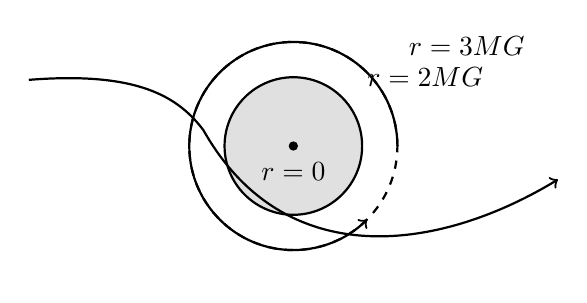
\begin{tikzpicture}[scale=1.12]
\fill[black!12] (0,0) circle (0.78);
\draw[thick] (0,0) circle (0.78);
\draw[dashed,thick] (0,0) circle (1.18);
\fill (0,0) circle (1.5pt);
\draw[->,thick] (1.18,0) arc (0:315:1.18);
\draw[->,thick] (-3.0,0.75)
  .. controls (-1.75,0.85) and (-1.30,0.55) .. (-1.02,0.18)
  .. controls (-0.10,-1.45) and (1.65,-1.20) .. (3.0,-0.38);
\node[right] at (0.73,0.78) {\(r=2MG\)};
\node[right] at (1.20,1.13) {\(r=3MG\)};
\node[below] at (0,-0.08) {\(r=0\)};
\end{tikzpicture}
\caption{Chân trời, mặt cầu photon và một tia bị lệch mạnh. Các tia gần quỹ đạo tròn không ổn định đến mức tùy ý có thể tích lũy độ lệch lớn đến mức tùy ý trước khi thoát ra hoặc rơi vào trong.}
\end{figure}

\begin{classroomqa}
\audiencequestion{Tại sao phải giữ cố định mômen động lượng, và nó liên hệ thế nào với tần số của một photon và quỹ đạo đi vào của nó?}
\lecturerresponse{Mỗi tia đều mang một mômen động lượng được bảo toàn đối với hố đen. Tần số của nó ấn định độ lớn của động lượng tuyến tính, còn độ lệch của nó khỏi tâm góp phần xác định \(L\). Ngoài một quỹ đạo tròn, có thể chọn bán kính và mômen động lượng một cách độc lập. Việc đòi hỏi một quỹ đạo tròn của photon gắn chuyển động với bán kính duy nhất \(3MG\), và sự phân tích thành nhân tử trong phương trình~\eqref{eq:l6-photon-energy} cho thấy bán kính này không phụ thuộc vào độ lớn của \(L\).
\lecturetimestamp{00:54:43--00:57:02}}
\end{classroomqa}

\begin{classroomqa}
\audiencequestion{Vì sao cực đại của năng lượng lại xác định một quỹ đạo?}
\lecturerresponse{Sau khi đã khử chuyển động góc tại \(L\) cố định, hàm còn lại đóng vai trò của một năng lượng hiệu dụng theo bán kính. Một điểm dừng cho cân bằng theo phương bán kính. Cực tiểu sẽ là ổn định; điểm này là cực đại và vì thế cho một quỹ đạo tròn không ổn định. Không có mâu thuẫn nào khi đồng thời gọi nó là cân bằng và không ổn định.
\lecturetimestamp{00:57:51--00:58:54}}
\end{classroomqa}

Một hạt có khối lượng có thể có các quỹ đạo tròn loại thời ở ngoài \(3MG\), dù những quỹ đạo gần mặt cầu photon nhất là không ổn định. Một hạt không khối lượng chỉ có quỹ đạo tròn tại \(3MG\). Bên trong mặt cầu photon, một photon chuyển động theo tiếp tuyến sẽ rơi vào trong; một vật chuyển động chậm hơn cũng không có cơ may nào tốt hơn để duy trì quỹ đạo như vậy. Phát biểu này liên quan đến chuyển động góc. Ở ngoài chân trời, một tia có hướng đủ ra ngoài vẫn có thể thoát ra ngay cả khi bán kính xuất phát của nó nhỏ hơn \(3MG\).

\section{Hố đen tác động lên ảnh như thế nào}

Mặt cầu photon giải thích vì sao lỗ đen không chỉ đơn thuần là một đĩa tối dán đè lên một bầu trời vốn dĩ không hề thay đổi. Ánh sáng từ một vật thể ở hậu cảnh có thể tới người quan sát theo nhiều đường đi. Một tia có thể đi qua một phía của lỗ đen, một tia khác qua phía bên kia, và những tia khác nữa có thể quay quanh nó một hoặc nhiều vòng. Kết quả có thể bao gồm các ảnh bị dịch chuyển, các ảnh bị nhân đôi, các vành, và một dãy vô hạn những ảnh ngày càng nhỏ hơn, ngày càng mờ hơn, ứng với những vòng quấn thêm. Bức tranh chính xác thì phức tạp, nhưng nguồn gốc của nó đã được hàm chứa ngay trong quỹ đạo không ổn định.

Khi nguồn, thấu kính và người quan sát thẳng hàng đủ tốt, ảnh có thể tạo thành một vành Einstein. Các vành do thấu kính hấp dẫn đã được quan sát trong tự nhiên. Ảnh đầy đủ của hố đen đòi hỏi phải tích phân các đường trắc địa null cho nhiều hướng ban đầu, một phép tính rất thích hợp để giao cho máy tính.

\begin{classroomqa}
\audiencequestion{Biên quang học này nói tới mặt cầu photon hay chân trời?}
\lecturerresponse{Chúng giữ những vai trò khác nhau. Chân trời tại \(2MG\) là biên nhân quả: không tín hiệu hướng tương lai nào thoát ra được từ bên trong nó. Mặt cầu photon tại \(3MG\) chi phối chuyển động theo tiếp tuyến và hiện tượng thấu kính mạnh. Giữa hai bán kính ấy, một tia hướng tâm đi ra ngoài có thể thoát ra, trong khi một tia tiếp tuyến thì rơi vào. Các hướng trung gian có thể lặp vòng trước khi thoát ra hoặc bị bắt giữ.
\lecturetimestamp{01:02:47--01:03:40}}
\end{classroomqa}

\begin{classroomqa}
\audiencequestion{Có thể tính một quỹ đạo ánh sáng tổng quát thay vì chỉ phác thảo nó không?}
\lecturerresponse{Có. Đưa điều kiện null vào các phương trình trắc địa hoặc Euler--Lagrange rồi tích phân với dữ liệu ban đầu đã chọn. Các phương trình ấy không mới về mặt khái niệm, nhưng việc truy vết tia lại rối rắm về đại số, nên tính toán số là phương pháp thực tế để dựng một ảnh.
\lecturetimestamp{01:03:48--01:04:27}}
\end{classroomqa}

\begin{classroomqa}
\audiencequestion{Nếu áp dụng trực tiếp các phương trình Euler--Lagrange thì phép tính quỹ đạo tròn có khó hơn không?}
\lecturerresponse{Nó sẽ cho cùng một kết quả. Tác dụng là điểm xuất phát thích hợp trong cả hai cách, nhưng các tọa độ chu kỳ làm lộ ra năng lượng và mômen động lượng bảo toàn. Dùng các hằng số đó trước là con đường ngắn hơn để đi đến điều kiện quỹ đạo tròn.
\lecturetimestamp{01:04:33--01:05:49}}
\end{classroomqa}

\section{Metric gần chân trời là không gian Rindler}

Bây giờ ta quay lại chân trời. Các hệ số Schwarzschild dường như phân kỳ hoặc triệt tiêu tại đó, và khi đi qua chân trời thì dấu của chúng đổi chỗ cho nhau. Tuy vậy, một quan sát viên rơi vào không gặp độ cong cục bộ phân kỳ nào tại mặt đó. Nguyên lý tương đương cho ta biết vì sao cả hai mệnh đề đều có thể đúng.

Bắt đầu với không-thời gian Minkowski hai chiều:
\begin{equation}
d\tau^{2}=dT^{2}-dX^{2}.
\end{equation}
Trong miền nêm Rindler bên phải, đặt
\begin{equation}
X=\rho\cosh\omega,
\qquad
T=\rho\sinh\omega.
\label{eq:l6-rindler-map}
\end{equation}
Các đường có \(\rho\) không đổi thỏa
\begin{equation}
X^{2}-T^{2}=\rho^{2},
\end{equation}
nên chúng là các hypebol, tức các đường thế giới của những quan sát viên gia tốc đều.
Thay phương trình~\eqref{eq:l6-rindler-map} vào metric phẳng, ta được
\begin{equation}
d\tau^{2}
=\rho^{2}d\omega^{2}-d\rho^{2}.
\label{eq:l6-rindler-metric}
\end{equation}
Bây giờ đặt
\begin{equation}
\rho^{2}=4\xi,
\qquad
\omega=\frac{t}{2}.
\label{eq:l6-rindler-rescale}
\end{equation}
Vì \(d\rho^{2}=d\xi^{2}/\xi\) nên phương trình~\eqref{eq:l6-rindler-metric}
trở thành
\begin{equation}
d\tau^{2}
=\xi\,dt^{2}-\frac{d\xi^{2}}{\xi}.
\label{eq:l6-xi-metric}
\end{equation}

\begin{classroomqa}
\audiencequestion{Các tọa độ góc hay tọa độ ngang đã đi đâu?}
\lecturerresponse{Chúng chỉ bị lược đi thôi. Ta đang khảo sát mặt phẳng cục bộ \(t\)-\(r\) chứa hành vi băng qua chân trời. Hai phương ngang vẫn đều đặn và có thể khôi phục lại; chúng không làm thay đổi kỳ dị tọa độ đang được phân tích.
\lecturetimestamp{01:16:27--01:16:47}}
\end{classroomqa}

Để so sánh với Schwarzschild, hãy chọn đơn vị sao cho \(2MG=1\). Phần theo bán kính của phương trình~\eqref{eq:l6-schwarzschild} là
\begin{equation}
d\tau^{2}
=
\frac{r-1}{r}\,dt^{2}
-
\frac{r}{r-1}\,dr^{2}.
\end{equation}
Rất gần \(r=1\), tử số nhỏ \(r-1\) phải được giữ lại, còn các thừa số \(r\) vốn vô hại ở những chỗ khác thì có thể thay bằng 1. Do đó
\begin{equation}
d\tau^{2}
\simeq
(r-1)\,dt^{2}
-
\frac{dr^{2}}{r-1}.
\end{equation}
Với
\begin{equation}
\xi=r-1,
\end{equation}
thì đây chính là phương trình~\eqref{eq:l6-xi-metric}. Hình học Schwarzschild gần chân trời, một cách cục bộ, là mô tả Rindler của không-thời gian phẳng.

\begin{classroomqa}
\audiencequestion{Làm sao đây có thể là các tọa độ gia tốc nếu không-thời gian nền là phẳng?}
\lecturerresponse{Gia tốc thuộc về quan sát viên, không nhất thiết thuộc về độ cong. Một đường thế giới tại \(\rho\) cố định là gia tốc đều trong không-thời gian Minkowski. Tương tự, một quan sát viên bị giữ ở bán kính cố định gần hố đen phải được đỡ để chống lại rơi tự do. Nguyên lý tương đương làm cho các mô tả cục bộ trùng khớp dù không-thời gian Schwarzschild hoàn chỉnh là cong.
\lecturetimestamp{01:22:19--01:24:06}}
\end{classroomqa}

\section{Băng qua chân trời Rindler}

Các công thức cho miền nêm phải chỉ bao phủ \(\xi>0\):
\begin{equation}
X=2\sqrt{\xi}\cosh\frac{t}{2},
\qquad
T=2\sqrt{\xi}\sinh\frac{t}{2}.
\label{eq:l6-rindler-outside}
\end{equation}
Mặt \(\xi=0\) là đường null \(X=T\). Để tiếp tục sang miền nêm tương lai, đặt
\begin{equation}
\zeta=-\xi>0
\end{equation}
và hoán đổi vai trò của các hàm hyperbol:
\begin{equation}
T=2\sqrt{\zeta}\cosh\frac{t}{2},
\qquad
X=2\sqrt{\zeta}\sinh\frac{t}{2}.
\label{eq:l6-rindler-inside}
\end{equation}
Metric vẫn là
\begin{equation}
d\tau^{2}
=\xi\,dt^{2}-\frac{d\xi^{2}}{\xi},
\end{equation}
nhưng khi \(\xi<0\), hệ số của \(dt^{2}\) là âm còn hệ số của \(d\xi^{2}\) là dương. Tọa độ \(\xi\), và do đó là phương bán kính Schwarzschild, đã trở thành loại thời; \(t\) đã trở thành loại không gian.

\begin{figure}[htbp]
\centering
\includegraphics[width=0.88\textwidth]{lecture_06_figure_06.png}
\caption{Các miền nêm Rindler, các biên null của chúng, và phép tiếp tục từ \(\xi>0\) sang \(\xi<0\). Trên bảng cũng ghi \(\rho^{2}=4\xi\) và \(\omega=t/2\).}
\lectureframe{01:29:40}
\end{figure}

\begin{classroomqa}
\audiencequestion{Có phải một số đường trong hình vẽ tọa độ này chuyển động nhanh hơn ánh sáng không?}
\lecturerresponse{Một đường lưới tọa độ không nhất thiết là đường thế giới của một vật chất. Độ dốc tọa độ của nó có thể trông như siêu quang mà không vi phạm nhân quả. Các tia sáng vật lý vẫn nằm trên các đường null, còn các hạt vật lý vẫn nằm bên trong các nón ánh sáng cục bộ của chúng.
\lecturetimestamp{01:28:44--01:29:08}}
\end{classroomqa}

Tiếp tục đi sâu hơn vào phần bên trong Schwarzschild cuối cùng sẽ đưa ta đến \(r=0\). Biên đó là loại không gian. Vì vậy mô tả nó như một thời điểm thì đúng hơn là như một nơi chốn: mọi quỹ đạo loại thời hay null hướng tương lai trong phần bên trong hố đen đều đi tới đó. Người ta có thể đi vòng quanh một nơi. Không thể đi vòng qua tương lai của chính mình.

\begin{classroomqa}
\audiencequestion{Liệu hình vẽ có thể đơn giản tiếp tục xuyên qua \(r=0\) tới \(r\) âm, và \(r=0\) có còn là tâm không?}
\lecturerresponse{Hình vẽ tọa độ có thể khiến ta muốn kéo dài một đường, nhưng nghiệm Schwarzschild cổ điển kết thúc tại kỳ dị độ cong. \(r=0\) vẫn có thể được gọi là tâm, nhưng đó là một tâm rất khác thường: ở bên trong, nó là một biên tương lai loại không gian. Không có sự đi qua chính quy nào xuyên qua đó tới một miền bán kính âm.
\lecturetimestamp{01:32:16--01:34:06}}
\end{classroomqa}

\begin{classroomqa}
\audiencequestion{Các trục chéo trong giản đồ Rindler có phải là loại ánh sáng không, và một vật rơi vào có thể đi vào tại một giá trị hữu hạn của thời gian gia tốc không?}
\lecturerresponse{Đúng, các biên của miền nêm là những đường null. Một đường thế giới rơi tự do cắt một đường như vậy tại một sự kiện hữu hạn hoàn toàn bình thường và trong một thời gian riêng hữu hạn. Tọa độ gia tốc \(t\), hay tương đương là \(\omega\), chạy ra vô hạn dọc theo mô tả bên ngoài với \(\rho\) không đổi; chính phép gán tọa độ ấy, chứ không phải sự kiện băng qua, mới trở nên vô hạn.
\lecturetimestamp{01:34:26--01:35:03}}
\end{classroomqa}

\section{Alice ở bên ngoài và Bob rơi vào}

Hãy để Alice ở bên ngoài tại bán kính cố định, được giữ lại để chống trọng lực, còn Bob thì rơi tự do. Gần chân trời, Alice đi theo một hypebol kiểu Rindler. Các lát \(t\) không đổi của cô dồn ngày càng sát biên null. Mọi sự kiện trên đường thế giới của Bob mà Alice gán cho một \(t\) hữu hạn đều nằm ngoài chân trời, nên cô ấy không bao giờ gán một thời gian Schwarzschild hữu hạn cho lần anh ấy băng qua.

Bob mang theo một chiếc đồng hồ đo thời gian riêng. Quỹ đạo của anh cắt qua đường null trong một khoảng hữu hạn trên chiếc đồng hồ ấy. Không có gì phân kỳ theo nghĩa cục bộ xảy ra khi anh băng qua. Chân trời có tính quyết định về mặt toàn cục nhưng về mặt cục bộ thì bình thường.

\begin{figure}[htbp]
\centering
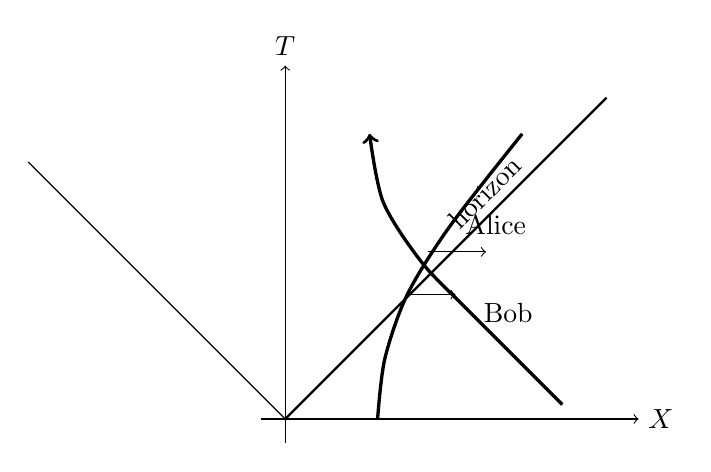
\begin{tikzpicture}[scale=1.02]
\draw[->] (-0.3,0) -- (4.4,0) node[right] {\(X\)};
\draw[->] (0,-0.3) -- (0,4.4) node[above] {\(T\)};
\draw[thick] (0,0) -- (4.0,4.0);
\draw[thin] (0,0) -- (-3.2,3.2);
\node[rotate=45,above] at (2.65,2.65) {horizon};
\draw[very thick]
  plot[smooth] coordinates {(1.15,0.0) (1.24,0.75) (1.52,1.55)
  (2.05,2.40) (2.95,3.55)};
\node[right] at (2.12,2.42) {Alice};
\draw[very thick,->]
  plot[smooth] coordinates {(3.45,0.18) (2.85,0.78) (2.25,1.38)
  (1.70,1.95) (1.22,2.70) (1.05,3.55)};
\node[right] at (2.35,1.32) {Bob};
\draw[->] (1.52,1.55) -- (2.12,1.55);
\draw[->] (1.78,2.08) -- (2.50,2.08);
\end{tikzpicture}
\caption{Đường thế giới được gia tốc của Alice ở bên ngoài và đường thế giới rơi tự do của Bob. Các lát tọa độ của Alice tiến gần đến chân trời; Bob băng qua nó trong thời gian riêng hữu hạn.}
\end{figure}

\begin{classroomqa}
\audiencequestion{Bob thấy gì khi ngoái lại nhìn Alice, và điều gì xảy ra với đồng hồ của anh sau khi băng qua?}
\lecturerresponse{Bob thấy Alice lùi xa với gia tốc cần thiết để giữ cô ở bên ngoài, nhưng anh không thấy một biến cố kỳ dị tại lúc mình băng qua. Alice có thể được giữ tại bán kính cố định; một quỹ đạo là một cách bố trí khả dĩ khác. Đồng hồ của Bob tiếp tục đo thời gian riêng \(\tau\) của anh một cách bình thường. Ở bên trong, việc nói rằng tọa độ bán kính là kiểu thời gian mô tả hình học nhân quả; điều đó không có nghĩa là chiếc đồng hồ đeo tay của anh theo nghĩa đen biến thành một thước mét. Đường thế giới của anh cuối cùng kết thúc tại \(r=0\).
\lecturetimestamp{01:39:51--01:44:45}}
\end{classroomqa}

Đường null giờ đây được nhận ra là chính chân trời, chứ không chỉ đơn thuần là một điểm nơi một hệ số tọa độ ứng xử bất thường. Bên ngoài nó, một họ tia sáng theo phương bán kính đi ra ngoài. Bên trong nó, cả hai hướng của nón ánh sáng tương lai đều dẫn tới \(r\) nhỏ hơn. Mọi quỹ đạo định hướng tương lai của vật có khối lượng đều phải nằm giữa các hướng null đó và vì thế đi tới điểm kỳ dị.

\section{Tín hiệu, sự dịch đỏ và một chân trời đang hình thành}

Giả sử vật chất đang suy sập phát ra một chuỗi đều đặn các xung ánh sáng. Một quan sát viên ở xa nhận các xung về sau với những khoảng thời gian ngày càng dài. Tần số của chúng dịch từ vùng khả kiến sang hồng ngoại, vi ba, vô tuyến và các bước sóng còn dài hơn nữa. Trong một phép tính cổ điển lý tưởng hóa, quan sát viên bên ngoài vẫn có thể tiếp tục liên hệ các tín hiệu ngày càng muộn hơn với vật chất đang tiến gần chân trời, nhưng trên thực tế nguồn nhanh chóng trở nên quá đỏ và quá mờ để phát hiện.

\begin{classroomqa}
\audiencequestion{Trong quá trình suy sập, một quan sát viên bên ngoài có thấy toàn bộ vật chất đơn giản là đóng băng tại chân trời không?}
\lecturerresponse{Trong thời gian Schwarzschild, bề mặt của vật chất đang suy sập tiến gần đến chân trời một cách tiệm cận và có vẻ ngày càng bị đóng băng. Điều thật sự được quan sát được mã hóa trong các tín hiệu ánh sáng, và các tín hiệu ấy ngày càng trễ hơn, dịch đỏ hơn và mờ hơn. Mô tả theo tọa độ này không nói rằng vật chất đang rơi vào trải qua một thời gian riêng vô hạn.
\lecturetimestamp{01:47:06--01:48:11}}
\end{classroomqa}

\begin{classroomqa}
\audiencequestion{Một quan sát viên ở thời điểm đủ muộn có thể khôi phục toàn bộ lịch sử của sự rơi hay không?}
\lecturerresponse{Chỉ thông qua những tín hiệu đã được phát ra và tới được quan sát viên. Các xung liên tiếp ngày càng cách xa nhau hơn và bị dịch đỏ mạnh hơn. Một quan sát viên lý tưởng với độ nhạy không giới hạn có thể theo dõi tín hiệu cổ điển tới các bước sóng ngày càng dài; một quan sát viên thực tế chỉ thấy vật thể mờ dần.
\lecturetimestamp{01:48:13--01:52:00}}
\end{classroomqa}

\begin{classroomqa}
\audiencequestion{Nói chính xác thì có ý gì khi bảo rằng điểm kỳ dị là một thời gian chứ không phải một nơi chốn?}
\lecturerresponse{Bề mặt \(r=0\) là kiểu không gian. Một khi đã ở bên trong chân trời, mọi đường cong kiểu thời gian hoặc null định hướng tương lai đều kết thúc ở đó. Một vị trí trong không gian có thể tránh được bằng cách chọn một lộ trình khác; còn một biên tương lai thì không thể tránh được nếu vẫn tiếp tục dọc theo một đường thế giới định hướng tương lai.
\lecturetimestamp{01:52:02--01:53:10}}
\end{classroomqa}

Vậy thì, nếu quan sát viên bên ngoài không bao giờ thấy vật chất đi qua, lỗ đen có thể hình thành hoặc tăng khối lượng bằng cách nào? Hãy xét một vỏ cầu đang suy sập. Chân trời toàn cục không chờ sẵn như một bề mặt vật chất có từ trước tại một bán kính cố định. Nó bắt đầu ở tâm và lớn dần ra ngoài, gặp vỏ đang suy sập khi vùng lỗ đen hình thành. Mô tả Schwarzschild bên ngoài vẫn làm cho vỏ tiến gần đến chân trời cuối cùng một cách tiệm cận. Bức tranh không-thời gian đầy đủ, kể cả cách chân trời được xác định một cách toàn cục, là chủ đề của bài giảng tiếp theo.

\begin{figure}[htbp]
\centering
\includegraphics[width=0.90\textwidth]{lecture_06_figure_07.png}
\caption{Một vỏ đang suy sập và chân trời lớn dần ra ngoài từ tâm để gặp nó. Hình vẽ này là phần xem trước của hình học suy sập toàn cục sẽ được phát triển trong bài giảng tiếp theo.}
\lectureframe{01:57:25}
\end{figure}

\begin{classroomqa}
\audiencequestion{Nếu trong thời gian tọa độ bên ngoài không có gì đi qua chân trời, thì lỗ đen có thể hình thành hoặc lớn lên như thế nào?}
\lecturerresponse{Tiền đề đó trộn lẫn một mệnh đề theo tọa độ với một mệnh đề toàn cục. Vật chất đang suy sập đi tới vùng liên quan trong thời gian riêng hữu hạn, còn chân trời sự kiện được xác định bởi cấu trúc nhân quả của toàn bộ không-thời gian. Trong bức tranh vỏ, nó bắt đầu ở tâm và lớn dần ra ngoài để gặp vỏ. Cái nhìn bị trễ và bị dịch đỏ của quan sát viên bên ngoài vẫn phù hợp với chân trời toàn cục đó.
\lecturetimestamp{01:53:11--01:57:34}}
\end{classroomqa}

\section{Các hướng thoát giữa hai mặt cầu}

Chân trời và mặt cầu photon chia bài toán tia sáng thành những trường hợp riêng biệt. Ở bán kính
\begin{equation}
2MG<r<3MG,
\end{equation}
một tia sáng đi ra theo phương bán kính có thể thoát tới vô cực. Một tia sáng tiếp tuyến thì không thể; nó rơi vào trong. Giữa các hướng đó là một nón thoát. Càng gần chân trời, nón ấy càng thu hẹp quanh hướng bán kính đi ra ngoài. Sau khi vượt qua chân trời, nó khép lại hoàn toàn.

\begin{classroomqa}
\audiencequestion{Một nguồn sáng nằm giữa chân trời và mặt cầu photon có thể gửi tín hiệu nào đó ra ngoài không?}
\lecturerresponse{Có. Một tia null đi ra ngoài đủ gần phương bán kính sẽ thoát được miễn là sự kiện phát của nó nằm ngoài \(2MG\). Phát biểu rằng chuyển động theo góc ở bên trong \(3MG\) rơi vào trong không cấm sự thoát theo phương bán kính. Kết cục phụ thuộc vào hướng phát, và nón đi ra ngoài được phép sẽ thu hẹp lại khi nguồn tiến gần chân trời.
\lecturetimestamp{01:57:34--01:59:48}}
\end{classroomqa}

\begin{classroomqa}
\audiencequestion{Một tia đi từ bên ngoài vào có thể đi vào bên trong mặt cầu photon, quay đầu lại và lại đi ra được không?}
\lecturerresponse{Không, nếu nó đi dọc theo một trắc địa null thuộc kiểu đang được bàn tới. Một điểm ngoặt sẽ có vận tốc bán kính bằng không, nên tia ấy trong khoảnh khắc sẽ là tiếp tuyến tại một bán kính nhỏ hơn \(3MG\); ở đó quỹ đạo theo góc rơi vào trong thay vì quay ngược ra ngoài. Tuy vậy, một nguồn đã ở giữa hai mặt cầu vẫn có thể phát ra một tia đi ra ngoài đủ gần phương bán kính trước khi nó vượt qua chân trời.
\lecturetimestamp{01:59:49--02:01:27}}
\end{classroomqa}

Câu hỏi cuối cùng này được cố ý để ngỏ hơn. Hãy hình dung Alice và Bob đều được giữ tại cùng một bán kính bên ngoài chân trời. Những quan sát viên ở gần nhau rõ ràng có thể trao đổi tín hiệu. Nếu họ cách xa nhau dọc theo mặt cầu, thì đường đi null trực tiếp và miền góc giới hạn của nó đòi hỏi một phép tính trắc địa tường minh. Lớp học đề xuất một lộ trình gián tiếp: gửi thông điệp gần như theo phương bán kính ra ngoài tới một trạm chuyển tiếp ở bán kính an toàn hơn, đem nó đi vòng quanh tại đó, rồi gửi ngược vào trong. Một phiên bản khác để cho một vật hoặc tín hiệu được ném ra ngoài quay đầu và quay trở lại. Những lộ trình này cho thấy vì sao việc không có một quỹ đạo tròn tiếp tuyến không tự nó cấm mọi sự liên lạc giữa các quan sát viên ở bên ngoài.

\begin{classroomqa}
\audiencequestion{Hai quan sát viên được treo tại cùng một bán kính gần chân trời có thể liên lạc với nhau vòng quanh lỗ đen không?}
\lecturerresponse{Về mặt cục bộ, có. Đối với các quan sát viên cách xa nhau hoặc ở hai điểm đối diện qua tâm, giới hạn của đường đi trực tiếp đã không được triển khai trong bài giảng và không nên được nâng thành một định lý. Phần thảo luận trước hết để ngỏ câu hỏi về trắc địa theo góc đó, rồi lưu ý rằng một tín hiệu gián tiếp có thể đi gần như theo phương bán kính ra ngoài, được chuyển tiếp vòng quanh ở bán kính lớn hơn, và quay trở lại. Khi tiến gần chân trời, miền góc hữu ích trực tiếp thu hẹp dần, nhưng ở ngoài chân trời vẫn còn một lộ trình đi ra ngoài.
\lecturetimestamp{02:01:29--02:04:17}}
\end{classroomqa}

Bước tiếp theo là thay những phác họa gần chân trời này bằng hình học toàn cục của một vật thể suy sập và xem chính xác chân trời sự kiện lớn lên như thế nào.